% !TEX TS-program = XeLaTeX
\documentclass{ISCISC2020}

% تقریبا تمامی بسته‌های مورد نیاز برای یک مقاله در استایل فراخوانی شده است. اما در هر صورت در صورتی‌که می‌خواهید بسته‌ای را فراخوانی کنید به صورت زیر عمل کنید. مثلا ما در کد زیر دوبسته glossaries و tikz را فراخوانی کرده‌ایم.
\makeatletter
\bidi@BeforePackage{xepersian}{
% \RequirePackage{tikz}
% \RequirePackage{glossaries}
\RequirePackage{natbib}
}
\makeatother


% عنوان مقاله را در این قسمت وارد کنید. 
\title{
کرم موریس: اولین حمله سایبری بزرگ در اینترنت
}
\date{}
% اسامی نویسندگان و همچنین اطلاعات مربوط به آن‌ها را در این قسمت وارد کنید. 
\author[1]{محمدحسین عباسپور ۹۹۵۲۱۴۳۳}
\author[1]{فرزان رحمانی ۹۹۵۲۱۲۷۲}
\author[2]{ابوالفضل دیانت}

\affil[1]{
دانشجوی کارشناسی مهندسی کامپیوتر، دانشگاه علم و صنعت ایران، تهران،
آدرس پست الکترونیکی:m\_abbaspoor80@comp.iust.ac.ir
}
\affil[1]{

دانشجوی کارشناسی مهندسی کامپیوتر، دانشگاه علم و صنعت ایران، تهران، 
آدرس پست الکترونیکی: farzan\_rahmani@comp.iust.ac.ir
}
\affil[2]{
استادیار دانشکده مهندسی کامپیوتر، دانشگاه علم و صنعت ایران، تهران، آدرس پست الکترونیکی: adiyanat@iust.ac.ir
}

\begin{document}
\maketitle

\begin{abstract}
کرم موریس\LTRfootnote{Morris worm} یا کرم اینترنتی یکی از قدیمی‌ترین کرم‌های رایانه‌ای است که از طریق اینترنت توزیع شده است و اولین موردی است که توجه رسانه‌های اصلی را به خود جلب کرده است. این کرم منجر به اولین محکومیت جنایی در ایالات متحده بر اساس قانون تقلب و سوء استفاده رایانه ای\LTRfootnote{Computer Fraud and Abuse Act} در سال 1986 شد. این بدافزار توسط یک دانشجوی فارغ التحصیل در دانشگاه کورنل، رابرت تاپان موریس\LTRfootnote{Robert Tappan Morris}، نوشته شد و در ساعت 8:30 بعد از ظهر 2 نوامبر 1988، از شبکه موسسه فناوری ماساچوست\LTRfootnote{Massachusetts Institute of Technology network} راه اندازی شد.
% (\lr{Style}) برای کلمات انگلیسی  

\end{abstract}

\begin{keywords}
کرم موریس،
 حمله سایبری،
 اینترنت،
 بدافزار،
 امنیت رایانه،
 قانون کلاهبرداری و سوء استفاده رایانه ای.
\end{keywords}

\section{مقدمه}
رشد سریع اینترنت در اواخر دهه 1980 چالش های جدیدی را در امنیت رایانه به وجود آورد. یکی از مهم ترین رویدادها در این دوره انتشار کرم موریس بود، یک برنامه خود تکرارشونده که باعث اختلال گسترده شد و آسیب پذیری های سیستم های کامپیوتری متصل به هم را برجسته کرد.

کرم موریس که در 2 نوامبر 1988 توسط رابرت تاپان موریس منتشر شد، نقطه عطفی در تاریخ امنیت سایبری بود. گسترش سریع این کرم که به عنوان یک آزمایش بی ضرر برای اندازه گیری اندازه اینترنت در نظر گرفته شده بود، آسیب پذیری های حیاتی را در زیرساخت های اولیه شبکه آشکار کرد که پیامدهای قابل توجهی را به دنبال داشت و باعث پیشرفت در اقدامات امنیت سایبری شد.


\section{داستان جذاب و پند‌آموز کرم موریس}

% \subsection{آشنایی با فرآیند آپدیت ویندوز دیفندر}

در سال 1988، دنیای دیجیتال با بحرانی مواجه شد که مانند گذشته نبود. یک پروژه تحقیقاتی به ظاهر بی ضرر، کرمی که توسط رابرت تاپان موریس، دانشجوی فارغ التحصیل دانشگاه کرنل ایجاد شد، از کنترل خارج شد. این کرم که برای کشف قابلیت‌های اینترنت نوپا طراحی شده بود، به طور ناخواسته از آسیب‌پذیری‌ها در برنامه‌های پرکاربرد سوء استفاده کرد و به سرعت تکرار شد و باعث اختلال گسترده شد. برخلاف ویروس‌ها\LTRfootnote{Viruses}، که برای انتشار به اقدامات انسانی نیاز دارند، این کرم از طریق اتصالات شبکه خودتکثیر می‌شود و تخمین زده می‌شود 10 درصد از تمام ماشین‌های متصل به اینترنت آن زمان را آلوده کرده است که در آن زمان تعداد بسیار زیادی بود.


کرم موریس یک برنامه خود تکرارشونده بود که از آسیب‌پذیری‌های سیستم‌های یونیکس\LTRfootnote{Unix} برای انتشار در شبکه‌های رایانه‌ای استفاده می‌کرد. با این حال، به دلیل یک خطای کدنویسی، کرم به صورت نمایی تکثیر شد و باعث آسیب غیرمنتظره و گسترده شد.

کد این کرم شامل چندین مؤلفه بود. ابتدا، سعی کرد از یک آسیب پذیری در دیمون انگشتی\LTRfootnote{fingerd daemon} سوء استفاده کند که اجرای دستور از راه دور را امکان پذیر می کرد. اگر شکست می‌خورد، سعی می‌کرد از طریق ضعف در حالت دیباگ برنامه sendmail یونیکس به آن دسترسی پیدا کند. زمانی که کرم وارد یک سیستم می‌شد، یک درب پشتی نصب می‌کرد که کنترل از راه دور آینده را امکان‌پذیر می‌کرد و سپس به جستجوی میزبان‌های آسیب‌پذیرتر برای آلوده شدن می‌پرداخت.

گسترش سریع کرم موریس اختلالات قابل توجهی ایجاد کرد و بر حدود 6000 سیستم رایانه ای در سراسر اینترنت نوپا، از جمله ماشین‌ها در دانشگاه های بزرگ، تأسیسات نظامی و مراکز تحقیقاتی تأثیر گذاشت. سیستم‌ها از کار افتادند یا تا حد خزیدن کند شدند و بهره‌وری و تلاش‌های تحقیقاتی را با مشکل مواجه کردند.

تأثیر این کرم با توانایی آن در تکثیر سریع خود، مصرف منابع سیستم و مسدود کردن شبکه‌ها با ترافیک بیش از حد تقویت شد. خسارات ناشی از کرم موریس میلیون‌ها دلار تخمین زده شد که خطرات بالقوه بدافزارهای خودتکثیر شونده و آسیب‌پذیری سیستم‌های کامپیوتری متصل به هم را نشان می‌دهد.

%\begin{figure*}[t]
\begin{figure}[h]
	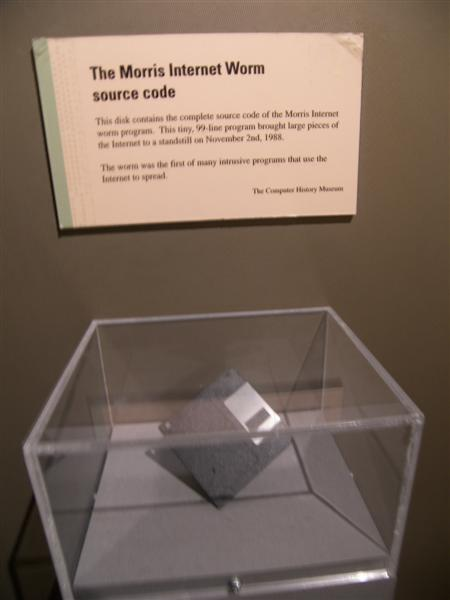
\includegraphics[width=\linewidth]{Images/Morris_Worm.jpg}
 	\caption{فلاپی دیسک حاوی کد منبع کرم موریس، در موزه تاریخ کامپیوتر\lr{[1]}}

\end{figure}
%\end{figure*}

% \subsection{آشنایی با فرآیند آپدیت ویندوز دیفندر}
داستان کرم موریس فقط در مورد هرج و مرج ناشی از آن نیست، بلکه در مورد واکنش زیبای آن نیز است. این حادثه شکنندگی اینترنت و نیاز به اقدامات امنیتی قوی را آشکار کرد. این امر باعث ایجاد دو موسسه مهم شد: مرکز هماهنگی CERT\LTRfootnote{CERT Coordination Center} (CERT/CC) در دانشگاه کارنگی ملون\LTRfootnote{Carnegie Mellon University} و گروه منطقه امنیتی نیروی ضربت مهندسی اینترنت(IETF)\LTRfootnote{Internet Engineering Task Force (IETF) Security Area Group}\lr{.} سازمان CERT/CC به عنوان یک منبع مرکزی برای هماهنگی تلاش‌های امنیت سایبری ظاهر شد، در حالی که IETF یک گروه اختصاصی برای رسیدگی به آسیب‌پذیری‌های امنیتی در پروتکل‌های اینترنتی ایجاد کرد.




% \subsection{آشنایی با فرآیند آپدیت ویندوز دیفندر}
شکار موریس کرم خود گواهی بر روحیه همکاری جامعه اولیه اینترنتی بود. با اطلاعات محدود و ابزارهای ابتدایی، محققان در سراسر جهان به طور خستگی ناپذیری برای درک رفتار کرم و شناسایی منبع آن تلاش کردند. چند روز پس از حمله، تیمی در دانشگاه برکلی کالیفرنیا\LTRfootnote{University of California, Berkeley}، کرم را به کامپیوتر موریس در کرنل ردیابی کردند که منجر به محاکمه و محکومیت نهایی او شد.

% \subsection{آشنایی با فرآیند آپدیت ویندوز دیفندر}
حادثه کرم موریس به عنوان یادآوری تلخ از تعادل ظریف بین نوآوری و امنیت است. این حادثه پیامدهای ناخواسته ای را که می تواند از اقدامات حتی با نیت خوب ناشی شود برجسته می کند و بر اهمیت همکاری در حفاظت از دنیای دیجیتال تأکید می کند. امروزه، امنیت سایبری به عنوان یک حوزه همیشه در حال توسعه باقی مانده است که دائماً با تهدیدات جدید و پیچیده دست و پنجه نرم می کند. با این حال، درس‌های آموخته‌شده از کرم موریس همچنان به توسعه اقدامات امنیتی قوی ادامه می‌دهد و تضمین می‌کند که اینترنت یک پلتفرم\LTRfootnote{platform} انعطاف‌پذیر و در دسترس برای اشتراک‌گذاری و اتصال دانش باقی می‌ماند.


\section{نتیجه گیری‌}
کرم موریس یک نقطه عطف مهم در تاریخ امنیت رایانه را رقم زد و آسیب پذیری های سیستم های متصل به هم و خطرات بالقوه بدافزارهای خود-تکثیر شونده را برجسته کرد. این حادثه راه را برای توسعه اقدامات امنیتی قوی تر و افزایش آگاهی از ملاحظات اخلاقی در برنامه نویسی رایانه ای هموار کرد. درس‌های آموخته‌شده از کرم موریس به تلاش‌های مداوم برای ایمن‌سازی اینترنت و محافظت از زیرساخت‌های حیاتی در برابر تهدیدات سایبری ادامه می‌دهد.

علاوه بر این، کرم موریس به عنوان یک رویداد مهم در تکامل امنیت سایبری است که به عنوان یک داستان هشدار دهنده و یک کاتالیزور برای نوآوری عمل می کند. با افشای آسیب‌پذیری‌ها در زیرساخت‌های اولیه اینترنت و ایجاد آگاهی گسترده از خطرات امنیت سایبری، راه را برای پیشرفت‌های قابل توجهی در این زمینه هموار کرد. میراث کرم موریس به عنوان یادآور ضرورت مستمر برای اولویت دادن به امنیت در یک چشم انداز دیجیتالی به طور فزاینده به هم پیوسته باقی می ماند.


\section*{سپاس‌گزاری}
از خداوند متعال بسيار سپاسگزاریم بابت توانی كه به مـا جهـت نوشـتن ايـن
مقاله اعطاء نمود. از جناب دكتر دیانت كه استاد ما در تهيه اين مقاله بوده‌اند
نيز بسيار تشكر ميكنیم. همچنين از خـانواده عزيـزمان كـه پشـتيبان و موجـب
دلگرمی ما هستند بينهايت سپاسگزاریم. 

% \bibliography{lib}
\section*{مراجع}

\begin{flushleft}
\lr{[1] Bardoc, Ylee. "Morris worm." Wikipedia, The Free Encyclopedia, en.wikipedia.org/wiki/Morris\_worm, 24 Nov. 2023, 22:49 UTC.}
\newline
\lr{[2] Vacca, J. R. (2017). Computer and Information Security Handbook (3rd ed.). Morgan Kaufmann.}
\newline
\lr{[3] Kizza, M. (2015). Guide to Computer Network Security (3rd ed.). Springer.}
\newline
\lr{[4] Hafner, K., \& Markoff, J. (1991). Cyberpunk: Outlaws and hackers on the computer frontier. Simon and Schuster.}
\newline
\lr{[5] Denning, P. J. (Ed.). (1990). Computers under attack: Intruders, worms, and viruses. Addison-Wesley Longman Publishing Co., Inc.}
\newline
\lr{[6] Orman, H. (2003). The Morris worm: A fifteen-year perspective. IEEE Security \& Privacy, 1(5), 35-43.}
\end{flushleft}

\theendnotes
\end{document}


